\subsection{UNISA}

Al realizar el experimento, se logró llegar al destino en el ttl 27. De estos, 4 no respondieron. Los ttls que Cimbala reconoció como intercontinentales fueron 6, 10, 12, 15, 17, 20, 21, 22 y 26.

\begin{figure}[!htbp]
  \centering
    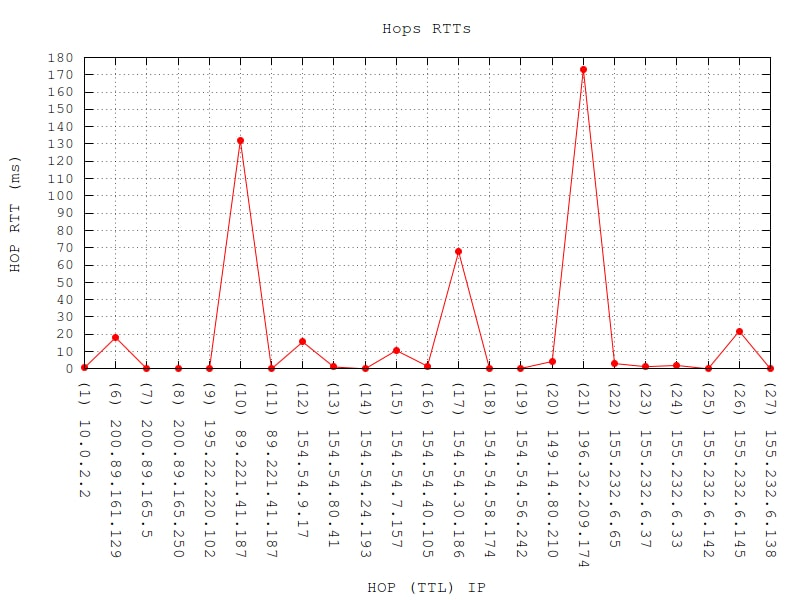
\includegraphics[scale=0.6]{imagenes/unisa-graficos/traceroute-unisa.jpg}
  \caption{UNISA- RTT hops}
  \label{fig:1}
\end{figure}

En la figura \ref{fig:1} se puede observar como el ttl 10, 17 y 21 tienen un rtt claramente distinguido del resto.

\begin{figure}[!htbp]
  \centering
    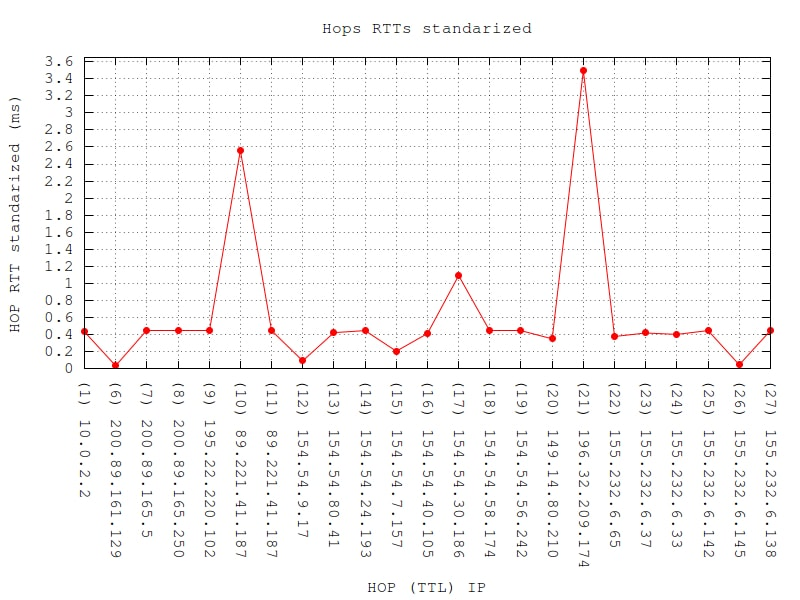
\includegraphics[scale=0.6]{imagenes/unisa-graficos/traceroute-unisa-standarized.jpg}
  \caption{UNISA- RTT hops standarized}
  \label{fig:2}
\end{figure}

En la figura \ref{fig:2} se puede observar una situacion similar a la de la figura \ref{fig:1}.

